% Section 6 (group C): the frame offset beta_sym and the counting rule (OP1)
\section{The frame offset \texorpdfstring{$\bsym$}{beta\_sym} and the counting rule (OP1)}
\label{sec:beta}

The numerical values that the construction offers for OP2--OP5 go back to one dimensionless number, the frame offset $\bsym\approx0.549$.
This section states how the number is defined, what it rests on, and what has been tried to derive it.  The short answer is that the
number is inserted, not derived: it is fixed by the ratio of two values of the Barbero--Immirzi parameter of loop quantum gravity, read as a Lorentz
factor.  Why two frames should use two different horizon counting rules is open problem OP1 \Open.  The structural routes to a frame-dependent
area quantum that the Companion has examined are closed; what remains is a choice.  Since 26 November 2026 the choice has a name and a status:
the author adopted the counting rule as a \emph{postulate} (\rnd{r67}), in the same sense as the exchange symmetry of Section~\ref{sec:B-koide}.
With it the number is computed from one rule with three named parts instead of being taken as the ratio of two literature values
(Section~\ref{sec:beta-postulate}).  The reason for the rule is still missing, and OP1 stays \Open.

\subsection{The number and its algebra}
\label{sec:beta-number}

Let $\gamma_{\mathrm{BI}}$ be the Barbero--Immirzi parameter from the horizon counting with all spins and weight two
(Domaga{\l}a--Lewandowski, Meissner \cite{DomagalaLewandowski2004,Meissner2004}) and $\gamma_{\mathrm{string}}=\ln2/(\pi\sqrt3)$ the value from the
counting with spin $j=\tfrac12$ only (Ashtekar, Baez, Corichi, Krasnov \cite{ABCK1998}).  The name ``string'' is historical; the value is the
ABCK count (\rnd{r24}, Remark~24.3).

\begin{proposition}[symmetric frame; \cite{QSC}, \texttt{thm:symmetric-frame}]
\label{prop:beta-symmetric}
Let $r>1$ and put $\beta:=\sqrt{(r-1)/(r+1)}$ and $\eta:=\operatorname{artanh}\beta$.  Then
\begin{equation}
 \frac{1+\beta^2}{1-\beta^2}=r=\cosh2\eta,\qquad
 \frac{2\beta}{1+\beta^2}=\tanh2\eta .
 \label{eq:beta-gL}
\end{equation}
Two observers at velocities $+\beta$ and $-\beta$ relative to a common frame therefore have mutual Lorentz factor $r$.
\end{proposition}

\begin{proof}
$(1+\beta^2)/(1-\beta^2)=\bigl((r+1)+(r-1)\bigr)/\bigl((r+1)-(r-1)\bigr)=r$.  With $\beta=\tanh\eta$ one has
$(1+\tanh^2\eta)/(1-\tanh^2\eta)=\cosh2\eta$ and $2\tanh\eta/(1+\tanh^2\eta)=\tanh2\eta$, the relativistic sum of $\beta$ and $\beta$.
\end{proof}

The algebra is \Established.  The physical content is the insertion
\begin{equation}
 r=\gamma_L:=\frac{\gamma_{\mathrm{BI}}}{\gamma_{\mathrm{string}}}=\frac{0.2375330}{0.1273840}=1.864700,\qquad
 \bsym=0.549406,\qquad \eta=0.6175,
 \label{eq:beta-values}
\end{equation}
which is \Conditional\ on reading a ratio of two values of one gravitational parameter as a Lorentz factor between the real projections of the
matter frame M and the tachyon frame T (\rndold{r61}, Theoremlet~61.1(c)).  (The main body of the Companion uses the rounded input $0.2375$, which gives $\bsym=0.549348$; \rndold{r63}.  From \rnd{r67} on the reference value is $\bsym=0.5494056410$, $\gamma_L=1.8646997646$; no recorded verdict depends on the difference.)  The ratio
$\gamma_L$ is $1/b_M$ in the register of Convention~F and the mutual Lorentz factor of two flux-opposed observers M and $\bar{\mathrm M}$; it is not a
boost between M and T, since a boost preserves $s=(E+iB)^2$ while the map to T reverses $\operatorname{Re}s$ (\rnd{r29}, Remark~29.4, read with $D$; \rnd{r64}.7).  In the
observer reading of the register (\rnd{r29}, Theoremlet~29.5), OP1 asks why M moves with $\bsym=0.5494$ relative to the rest frame of the field.

\subsection{The number as a ratio of two horizon counts}
\label{sec:beta-counting}

A horizon counting rule assigns a weight $g(j)$ to each spin $j\in\{\tfrac12,1,\tfrac32,\dots\}$ of a puncture.  With the area spectrum
$a(j)=\sqrt{j(j+1)}$, the Barbero--Immirzi parameter is the positive root of
\begin{equation}
 \sum_j g(j)\,e^{-2\pi\gamma\,a(j)}=1 .
 \label{eq:beta-counting}
\end{equation}
Table~\ref{tab:beta-rules} lists the three rules that matter here (\rndold{r63}, Theoremlet~63.1, rechecked in \rndold{r68}; the values agree
with Meissner's $0.23753295796592$ to the digits shown).

\begin{table}[ht]
\centering\small
\begin{tabular}{@{}llccc@{}}
\toprule
rule & source & $\gamma$ & $\gamma/\gamma_{\mathrm{string}}$ & $\beta$\\
\midrule
$j=\tfrac12$ only, $g=2$ & ABCK \cite{ABCK1998} & $0.1273840$ & $1$ & $0$\\
all $j$, $g=2$ (U(1)) & DL, Meissner \cite{DomagalaLewandowski2004,Meissner2004} & $0.2375330$ & $1.864700$ & $0.549406$\\
all $j$, $g=2j+1$ (SU(2)) & Ghosh--Mitra; ENP \cite{GhoshMitra2005,EngleNouiPerez2010} & $0.2740669$ & $2.151501$ & $0.604468$\\
\bottomrule
\end{tabular}
\caption{Counting rules and the resulting frame offset.  The lepton window $\beta\in[0.545,0.570]$ of \rndold{r61} contains, of these three, only the U(1)
pair.  Status: values \Established\ (numerical roots); their use as frame rules \Conditional.}
\label{tab:beta-rules}
\end{table}

Two facts weigh against the chosen pair.  First, it is a U(1) counting.  The SU(2)-invariant treatment of the horizon
\cite{EngleNouiPerez2010} is regarded in the literature as better founded; it gives $\gamma\approx0.274$ and $\bsym=0.604$, outside the window.
The data therefore select the counting that the later literature considers less well founded (\rndold{r68}, Correction~68.3).  Second, the
selection was made with the window in view (\rndold{r63} is marked not blind).

One mathematical fact supports the reading as a statement about states rather than about parameters.

\begin{proposition}[uncertainty saturation; \rndold{r63}, Theoremlet~63.2]
\label{prop:beta-saturation}
In the state $|j,m\rangle$ ($\hbar=1$) one has $\Delta J_x\,\Delta J_y=\tfrac12\bigl(j(j+1)-m^2\bigr)\ge\tfrac12|m|$, with equality exactly for
$m=\pm j$.  Hence at every $j$ exactly two states saturate the Robertson bound, and at $j=\tfrac12$ every state does.
\end{proposition}

\begin{proof}
$\langle J_x\rangle=\langle J_y\rangle=0$ and $\langle J_x^2\rangle=\langle J_y^2\rangle=\tfrac12\bigl(j(j+1)-m^2\bigr)$, while the Robertson bound is
$\tfrac12|\langle J_z\rangle|=\tfrac12|m|$.  The difference is $\tfrac12(j-|m|)(j+|m|+1)$, which vanishes iff $|m|=j$.
\end{proof}

The weight two of the M rule thus counts the extremal doublet $|j,\pm j\rangle$ at every $j$; Meissner's counting of labels $\pm m$ matches this
\cite{Meissner2004} (\rndold{r68}).  This is a reinterpretation of the U(1) counting, not part of its derivation \Reading.

\subsection{What depends on the rule}
\label{sec:beta-dependence}

The Companion keeps a list of its assumptions, each with an origin category; one category, ``R'', marks assumptions set after a consequence was known
(\rnd{r08}, Remark~8.2).  Bookkeeping of the four predictions open at that time shows that three of them rest on the same core (\rnd{r08}, Theoremlet~8.3):

\begin{center}\small
\begin{tabular}{@{}lll@{}}
\toprule
prediction & statement & inputs besides the literature values\\
\midrule
H96 & $\Omega_M=\bsym^2=0.30185$ & counting rule per frame, epoch ``today''\\
H15 & $m_W=m_Z\gamma_L/\sqrt{1+\gamma_L^2}$ & counting rule, reading $\cot\theta_W=\gamma_L$\\
H46 & $\sin^2\theta_{23}\in[0.49,0.50]$ & counting rule, neutrino reading, mask, $\varepsilon=\eta$\\
H42 & $\sin^2\theta_{23}\le0.54$ & neutrino reading, mask (independent of $\gamma_L$)\\
\bottomrule
\end{tabular}
\end{center}

If the counting rule fails, H15, H46 and H96 fail together.  With the SU(2) counting one would get $m_W=82.69$\,GeV and $\Omega_M=0.365$
instead of $80.361$\,GeV and $0.302$.  The U(1) rule was selected by the lepton window and the $m_W$ relation was noticed afterwards, so these
agreements are not independent of the selection.  The four predictions form two independent groups, not four; of those listed as open since
(Table~\ref{tab:open-tests}), H9 and H102 use the same number and H112 only the equality of two readouts.  Forming $\gamma_L$ without
a declared map from T to M is frame mixing in the sense of Convention~F: $\gamma_L$ is defined only through the reading it supports
(\rnd{r08}, item~8.3(d)).

\subsection{The special position of the pair (H98) and its limits}
\label{sec:beta-h98}

Test H98 asked how special the chosen pair is (\rnd{r09}, Theoremlet~9.1; pre-registered, \emph{not blind}: all three data values and the
agreement of the chosen pair were known).  The rule space has the spin ranges all $j$, half-integer $j$, integer $j\ge1$, $j=\tfrac12$ only and
$j=1$ only, with weights $2$ and $2j+1$: nine distinct rules and $36$ pairs with $\gamma_M>\gamma_T$.  Three windows were fixed: the lepton window
$\beta\in[0.545,0.570]$; $m_W$ within $2\sigma$ of the PDG 2025 average $80.3692\pm0.0133$\,GeV via $\cot\theta_W=\gamma_L$; and $\Omega_M$ within
$2\sigma$ of DESI DR2 BAO, $0.2975\pm0.0086$ \cite{DESIDR2}, via $\Omega_M=\beta^2$.  Two pairs fall in the lepton window, one in the $m_W$ window,
two in the $\Omega_M$ window, and exactly one in all three: all spins with weight two for M and $j=\tfrac12$ for T, with $\gamma_L=1.864700$,
$m_W=80.3615$\,GeV ($0.6\sigma$) and $\Omega_M=0.3018$ ($0.5\sigma$).  The SU(2) pair misses all three.  Figure~\ref{fig:beta-pairs} shows the
$36$ values.

\begin{figure}[t]
\centering
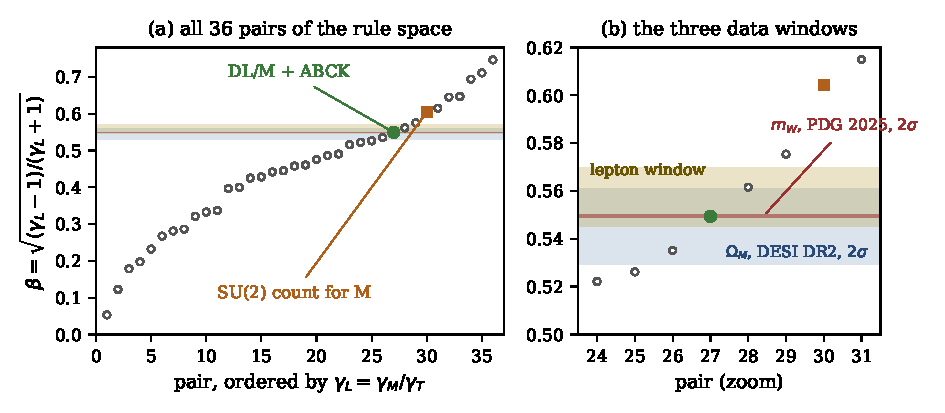
\includegraphics[width=\textwidth]{figures/F7-counting-pairs.pdf}
\caption{Frame offset $\beta=\sqrt{(\gamma_L-1)/(\gamma_L+1)}$ for the $36$ counting-rule pairs of the rule space of H98, ordered by
$\gamma_L=\gamma_M/\gamma_T$.  Filled circle: the pair DL/Meissner for M with ABCK for T; square: the SU(2) count ($g=2j+1$) for M with ABCK for
T.  Bands in (b): lepton window $[0.545,0.570]$, $\Omega_M=\beta^2$ within $2\sigma$ of DESI DR2 BAO, and $m_W$ within $2\sigma$ of PDG 2025
(narrow band).  Recomputed by \texttt{scripts/F7\_counting\_pairs.py} from the rule space of \rnd{r09} (script \texttt{k218}); the values agree with
its stored output.  Status: the confirmation of H98 is \emph{not blind}; with a free area spectrum the position is not unique (H104,
\Refuted), and the hits are compatible with chance once the selection of the pair is counted.}
\label{fig:beta-pairs}
\end{figure}

The weight of this result is limited in three ways.
\begin{enumerate}
\item Only the $m_W$ window selects uniquely, and the $m_W$ relation was itself found afterwards.  The $36$ values of $\gamma_L$ lie between
$1.006$ and $3.51$; the $m_W$ window is about $\pm0.003$ wide in $\gamma_L$, so about $0.08$ pairs would be expected in it.  A chance triple
agreement is of the order of a few per cent (\rnd{r09}).
\item The singular position depends on the fixed spectrum $\sqrt{j(j+1)}$.  With a free area spectrum (23 rules, 253 pairs), a second pair meets
all three windows ($\gamma_L=1.864824$).  The pre-registered test H104 is therefore \Refuted; H98 stays confirmed in its own rule space
(\rnd{r14}, Theoremlet~14.1).  A first run with a faulty solver had reported the opposite; it is disclosed in the Companion.
\item A chance estimate with a procedure fixed before the computation (\rnd{r30}, Remark~30.5) uses 16 targets, eight forms and a $2\sigma$ window.
The pair gives three hits ($\sin^2\theta_{12}$ and $\Omega_m$ by $\beta^2$, $\cot\theta_W$ by $\gamma_L$), the only pair of the 36 with three.  The
probability of at least three hits for a random $\gamma_L$ is $0.018$ to $0.023$; over 36 pairs the expected number is $0.64$ to $0.81$.  While the pair
is chosen rather than derived, the hits are compatible with chance.  The two targets near $0.30$ are strongly correlated, so two of the three hits
are nearly one.
\end{enumerate}

\subsection{Attempts to derive the assignment}
\label{sec:beta-attempts}

All attempts below are explorations \Exploration; their targets were known.

\paragraph{Energy and Unruh statistics.}
A principle was proposed in \rnd{r09} (Remark~9.2): a frame counts the states that saturate the uncertainty bound (P1) and are compatible with
its energy condition (P2), where T, as a tachyon relaxing to its floor (\rndold{r63}, Theoremlet~63.3), reaches only the smallest excitation.  P2 does
not survive.  By the local first law of isolated horizons \cite{FroddenGhoshPerez2013}, an observer at proper distance $\ell$ assigns a puncture of
area $8\pi\gamma a(j)$ ($\ell_P=1$) the energy $E_j=\gamma a(j)/\ell$ and has Unruh temperature $T_U=1/(2\pi\ell)$, so
\begin{equation}
 E_j/T_U=2\pi\gamma\,a(j),
 \label{eq:beta-unruh}
\end{equation}
independent of $\ell$.  Equation~\eqref{eq:beta-counting} is this Boltzmann statistics, and all static observers count alike (\rnd{r10},
Theoremlet~10.1).  The tachyon map commutes with the boost and fixes the vacuum, so an observer in T sees the same KMS state (Theoremlet~10.2).  The
tachyon floor is a property of a particle, not of the state seen at the horizon.

\begin{proposition}[the rule as an area quantum; \rnd{r10}, Theoremlet~10.3]
\label{prop:beta-area}
If M and T see the same statistics, the same geometry and both satisfy $S=A/4$, the assignment of counting rules is equivalent to a
frame-dependent Barbero--Immirzi parameter, $\gamma_M=\gamma_{\mathrm{BI}}$, $\gamma_T=\gamma_{\mathrm{string}}$: the smallest area quantum is smaller
by the factor $\gamma_L$ in T than in M, while the classical area and $G$ are the same.
\end{proposition}

This is an equivalence under stated assumptions \Conditional, not a reason.  The counting rule is from here on an assumption about a
frame-dependent area quantum.

\paragraph{Group theory of the readout.}
Assume (A) that the frame maps act on a puncture of spin $j$ through the same $SU(2)$ as on the field doublet $\chi$, i.e.\ as $e^{-i\pi J_k}$ about
three orthogonal axes.  Then they act irreducibly only for $j=\tfrac12$ (for half-integer $j$ they anticommute and the space splits into copies of
the doublet; for integer $j$ they commute), while the extremal doublet $|j,\pm j\rangle$ is invariant for every $j$.  The rules ``T counts punctures
on which the frame maps act irreducibly'' and ``M counts the invariant extremal doublet'' reproduce exactly the H98 pair (\rnd{r17},
Theoremlet~17.3; checked for $j\le20$).  In a strand picture (a spin-$j$ edge as a symmetrised bundle of $2j$ strands) bosonic strands give all $j$ and
fermionic strands only $j=\tfrac12$ (Theoremlet~17.5), but nothing in the frame or port structure distinguishes the statistics of strands
(\rnd{r24}, Theoremlet~24.1).  What remains is a reading \Reading: T counts crossings of the horizon, one crossing carrying one strand
(\rnd{r24}, Remark~24.4).  It replaces a placeholder (``T = string sector'') by a statement that refers to passages of the Companion (a narrative theorem and a typing), but it derives nothing.

\paragraph{Where the weakest point is.}
Every route to the assignment needs four parts: the area spectrum $\propto\sqrt{j(j+1)}$ (K0, from the literature), weight two for M (K1), all spins
for M (K2) and $j=\tfrac12$ only for T (K3).  Across six routes K0 is always set, K1 has partial supports, K2 none, and K3 only under (A) or explicit
placeholders (\rnd{r30}, Remark~30.4).  Of five reasons collected for the T rule none is free of the data (\rnd{r30}, Remark~30.3).  The rule of T
is a choice.

\paragraph{One number as a dimension.}
In units of the T quantum, equation~\eqref{eq:beta-counting} reads $\sum_j g(j)\,r_j^{D}=1$ with $r_j=2^{-a(j)/a(1/2)}$ and $D=\gamma/\gamma_T$: a
Moran equation of a self-similar set with $g(j)$ copies at scale $r_j$.  Then $D_T=1$, $D_M=\gamma_L=1.8647$ and $D_{\mathrm{SU(2)}}=2.1515$; the M set
fits in the plane and the SU(2) set cannot ($\sum(2j+1)r_j^2=1.199>1$) (\rnd{r29}, Theoremlet~29.3).  Reading the M rule as the richest such structure that fits on a surface is a reading stated afterwards.  A related exact statement: the weight two requires that the maps of $|j,+j\rangle$ and $|j,-j\rangle$
are distinct; if they coincide, or only one is admitted, the M rule falls to $\gamma_1=0.161586$ (\rnd{r53}, Theoremlet~53.2).  Weight two thus
asks for a readout that distinguishes the two orientations of a puncture without selecting one.

\subsection{Structural no-go results for a frame-dependent area quantum}
\label{sec:beta-nogo}

Proposition~\ref{prop:beta-area} asks for a map between frames that changes the area quantum by $\gamma_L$ at fixed $G$.  Three candidates have
been checked; none carries.

\paragraph{Unitary boosts.}
Rovelli and Speziale \cite{RovelliSpeziale2003} show that a boosted observer measures an area operator that does not commute with the original one;
if the boost acts unitarily, both have the same spectrum and the same smallest area, and only the distribution of eigenvalues changes.  Since M
and $\bar{\mathrm M}$ are related by a genuine boost, and the duality part $J_B$ leaves the geometry fixed, no decomposition of the frame map into
boost and duality yields a frame-dependent area quantum while the boost acts unitarily.  The assignment is compatible with standard loop quantum
gravity only if the map $\mathrm M\to\mathrm T$ is not unitary, the $J_B$ image with imaginary rapidity $i\pi/2$ being the only candidate, or if
$\gamma_T$ is read as a mean and not as an eigenvalue parameter, which is not a counting rule (\rnd{r30}, Remark~30.1).  A boost along the horizon normal prefers extremal states but does not select them (Remark~30.2).

\paragraph{Holst term and duality rotations.}
Write the gravitational Lagrangian of the action W1 with a Holst term \cite{Holst1996} as $L=A\langle\star\Sigma,R\rangle+B\langle\Sigma,R\rangle$
with $A=-1/(2\kappa)$ and $B/A=1/\gamma$.

\begin{proposition}[\rnd{r31}, Theoremlets~31.3 and 31.4]
\label{prop:beta-holst}
\textup{(a)} Real boosts, rotations and the complex boost with rapidity $\eta+i\pi/2$ leave $L$ invariant and do not change $\gamma$.
\textup{(b)} A duality rotation of the curvature, $R\mapsto\cos\theta\,R+\sin\theta\star R$, maps $(A,B)\mapsto(A\cos\theta+B\sin\theta,\;B\cos\theta-A\sin\theta)$,
hence $\arctan\gamma'=\arctan\gamma+\theta$.  \textup{(c)} Every sequence of such rotations preserves $A^2+B^2$.  Since the area quantum is
proportional to $\kappa\gamma=-1/(2B)$, for real results
\begin{equation}
 \frac{a'}{a}=\pm\sqrt{\frac{1+\gamma'^2}{1+\gamma^2}} ,
 \label{eq:beta-holst}
\end{equation}
so $\gamma_M\mapsto\gamma_T$ changes the area quantum by $\pm0.981$, not by the factor $\gamma_T/\gamma_M=0.536$ required at equal Newton constant.
\end{proposition}

\begin{proof}
(b) The pair $(A,B)$ is rotated by $-\theta$, and $\gamma'=A'/B'=(\gamma+\tan\theta)/(1-\gamma\tan\theta)=\tan(\arctan\gamma+\theta)$.  (c) Rotations
preserve the Euclidean norm of $(A,B)$.  With $A=\gamma B$,
\[
 A^2+B^2=B^2(1+\gamma^2)\quad\Longrightarrow\quad \frac{B}{B'}=\pm\sqrt{\frac{1+\gamma'^2}{1+\gamma^2}},
\]
and $\sqrt{(1+0.127384^2)/(1+0.237533^2)}=0.981$.  Part (a) and the absence of a distinguished angle ($\theta^*=-0.1065$) are checked in Wolfram
Language in the Companion.
\end{proof}

The only place in W1 plus Holst where a frame-dependent $\gamma$ can arise is a duality rotation of the curvature, which is not a symmetry of the
action; and it cannot produce $\gamma_L$ at equal $G$ by any path.  Part (c) was found afterwards; its algebra is elementary
\Established\ (within this action).

\paragraph{The non-unitary frame map $J_B$.}
$J_B$, conjugation with $\exp(i\tfrac\pi2K_x)$, is an automorphism of the Lorentz algebra, and conjugation by any invertible operator, unitary or not,
keeps every spectrum.  Reading the area in T through the transformed simplicity condition $K=\gamma L$ gives $\Gamma'=\operatorname{diag}(\gamma,-1/\gamma,-1/\gamma)$:
$\gamma$ along the M--T axis, $-1/\gamma$ across it.  At $\gamma_M$ this is $0.2375$ and $-4.2099$, matching neither $\gamma_T$ nor $\gamma_L$; the
pre-registered H121c is \Refuted\ (\rnd{r52}).  In the finite representations checked the complex boost is even unitary; questions of domain in
the infinite-dimensional unitary representations remain open.

With these three results the last structural candidate for a frame-dependent area quantum named in the Companion does not carry.  OP1 rests on the
assignment of the counting rules itself.

\subsection{A temporally ordered octant readout (H123)}
\label{sec:beta-h123}

Weight two asks for a readout that separates the two orientations of a puncture without selecting one.  The octant of Section~\ref{sec:B-koide} offers a candidate:
three readout windows in the order $R\to T\to J_B$ ($\tau=+1$) or reversed, on the extremal states of spin $j$ along $z$, $x$, $y$, with pole-sign
product $\varepsilon$ (\rnd{r58}; pre-registered, H123a--c not blind).

\begin{proposition}[\rnd{r58}, Theoremlets~58.1 and 58.2]
\label{prop:beta-octant}
The Bargmann invariant of the ordered triple is
\begin{equation}
 B_\tau=2^{-3j}\,e^{\,i\tau\varepsilon j\pi/2}.
 \label{eq:beta-bargmann}
\end{equation}
It gives the two orientations ($\varepsilon\mapsto-\varepsilon$) equal modulus and coincides for both exactly when $j\in\{2,4,6,\dots\}$.  The
temporally ordered readout therefore separates the orientations exactly for $j\notin2\mathbb N$.
\end{proposition}

\begin{proof}
Extremal states are spin-coherent states, so each overlap is the $2j$-th power of the spin-$\tfrac12$ overlap, and the spin-$\tfrac12$ triple has
modulus $2^{-3/2}$ and phase $\tau\varepsilon\pi/4$ (\rnd{r31}, Theoremlet~31.1).  The phases $e^{\pm ij\pi/2}$ agree iff $j\pi\in2\pi\mathbb Z$.
The Companion checks~\eqref{eq:beta-bargmann} exactly in 640 cases (Wolfram) and as a quantum circuit for $j=\tfrac12,1,2$ (Qiskit).
\end{proof}

Used as a counting rule, with weight two where the readout separates the orientations, weight one where it merges them, and T at $j=\tfrac12$,
the root of~\eqref{eq:beta-counting} is $\gamma_M'=0.2341229$, hence $\gamma_L'=1.837930$, $\beta'=0.543379$, $m_W'=80.0994$\,GeV ($-20.3\sigma$
from PDG 2025) and $\Omega_M'=0.2953$.  The lepton and $m_W$ windows are missed; H123d does not carry \Refuted\ (\rnd{r58}, Theoremlet~58.3).  The
readout sees the octant sign, not a weight two at every $j$.  Where the time direction $\tau$ comes from remains open.

\subsection{The counting rule as a postulate, and the two-readout reading}
\label{sec:beta-postulate}

\paragraph{The postulate (\rnd{r67}).}  (C1) In the matter frame M every spin $j\ge\tfrac12$ of a puncture counts with weight two, the extremal
doublet $m=\pm j$.  (C2) The area of a puncture is proportional to $\sqrt{j(j+1)}$.  (C3) The frame T counts only $j=\tfrac12$, and one such
puncture carries one bit.  The assignment of the two rules to M and T is part of the postulate.  It is adopted by the author as a working
assumption and is not derived \Conditional.

\begin{proposition}[the number that follows; \rnd{r67}, Theoremlet~67.1]
\label{prop:beta-postulate}
Under (C1)--(C3), with $k=2j$ and $c_k=\sqrt{k(k+2)/3}$, the factor $\gamma_L$ is the unique positive root of
\begin{equation}
 \sum_{k\ge1}2^{\,1-\gamma_Lc_k}=1,\qquad\text{so}\qquad \gamma_L=1.8646997646,\quad \bsym=0.5494056410 .
 \label{eq:beta-postulate}
\end{equation}
If (C2) is replaced by the semiclassical area $j+\tfrac12$ in both frames, the sum is geometric and $\gamma_L=2$, $\bsym=1/\sqrt3$ exactly.
\end{proposition}

\begin{proof}
Equation~\eqref{eq:beta-counting} with $g=2$ and $\gamma=\gamma_M$, written in units of the T quantum $\gamma_T=\ln2/(\pi\sqrt3)$, is
\eqref{eq:beta-postulate} with $\gamma_L=\gamma_M/\gamma_T$; the left side decreases strictly in $\gamma_L$.  With $c_k=(k+1)/2$ and
$x=2^{-\gamma_L/2}$ the sum is $2x^2/(1-x)$, which equals $1$ at $x=\tfrac12$.
\end{proof}

The proposition is \Established\ as a computation (root and ratio agree to $39$ digits, \texttt{mpmath} and Wolfram Language).  It shows where the
number comes from once the rule is granted.  It also shows where the physics sits: the difference between the Hopf value $1/\sqrt3$ of the
Companion (\texttt{thm:bsym-hopf}) and $\bsym$ is the difference between the area $j+\tfrac12$ and the Casimir area.  The value is not
fitted to data, but the windows of Section~\ref{sec:beta-dependence} were known when the rule was chosen, so the postulate is not a blind
prediction.

\paragraph{The two-readout reading (\rnd{r66}; tests H161, H164).}  Read the Hopf sphere of \texttt{thm:bsym-hopf} as the celestial sphere of light
directions; this reading is set \Reading.  Two null directions at angle $\theta$ have spinor overlap $\cos(\theta/2)$, and the boost with velocity
$\cos(\theta/2)$ along their bisector makes them antipodal.  For the pure Hopf state $K_1$ at the polar angle $\theta_H=2\arcsin\bsym$ and the
antipode $S$ of the photon pole this gives $|\langle K_1|S\rangle|=\bsym$: the angle reading and the velocity reading of $\bsym$ are one statement.
The boost has the rapidity $\eta$ of~\eqref{eq:beta-values}, and it carries the angle between the pole and $K_1$ from $\theta_H$ to $2\alpha$ with
$\cos2\alpha=1/\gamma_L$, so that the populations along the image of the pole are $(1,\bsym^2)/(1+\bsym^2)$, those of the matter state of Convention~F.
The equal mixture of the two readouts is not the matter state (Bloch length $\bsym$ against $1/\gamma_L$).  All of this holds identically in
$\beta$ and derives no value.

\paragraph{The overlap closure forces the Hopf value (\rnd{r67}; test H165).}  With spin $j$ carried by $2j$ symmetrised qubits, the coherent states
of the pair have overlap $\bsym^{2j}$, and
\begin{equation}
 \sum_{j\ge1/2}2\,|\langle j;K_1|j;S\rangle|^2=\frac{2\beta^2}{1-\beta^2}=\gamma_L-1
\end{equation}
for every $\beta$.  The closure ``sum $=1$'' holds exactly at $\beta=1/\sqrt3$.  The two-readout picture by itself therefore yields the Hopf value
and not $\bsym$; four further closures and thirteen number candidates fixed in advance give no identity either.  The pre-registered test H165
is \Refuted\ (predominantly not blind).  Two near coincidences at $5\cdot10^{-4}$ remain unexplained and are not used
($2^{1-\gamma_L}=0.549161$ against $\bsym$; \rnd{r67}, Remark~67.4).  A survey made for this test lists $37$ attempts in the Companion to derive
$\bsym$; none succeeds.

\subsection{One number, five translations}
\label{sec:beta-translations}

The numerical values used in OP2--OP5 all go back to $\bsym$.  The ways the number enters the sectors do not: they are five separate
identifications, four of them chosen after the data were known (\rnd{r30}, Remark~30.6).

\begin{center}\small
\begin{tabular}{@{}p{0.13\textwidth}p{0.36\textwidth}p{0.42\textwidth}@{}}
\toprule
problem & translation (set) & own remainder, independent of the number\\
\midrule
OP2 & spectral offset $=\bsym$ & existence and self-adjointness of the operator\\
OP3 & residual bend $\Phi_e=\pi/4-\gamma_M/2$ (H102) & origin of three generations, location of the bend\\
OP4 & $|U_{e2}|^2=\beta^2$ (H9); mask parameter $=\eta$ (H45/H46) & mask form, TM2, $\delta_{\mathrm{CP}}$, CKM\\
OP5 & $\Omega_M=\beta^2$ (H96) & mechanism selecting the ratio; absolute value of $\Lambda$\\
electroweak & $\cot\theta_W=\gamma_L$ (H15) & no $SU(2)\times U(1)$ in the observer reading\\
\bottomrule
\end{tabular}
\end{center}

A common origin of the five translations would require a mediator: one dimensionless output fixing $\eta$, a coupling of M and T through a state of
its own rather than a unitary frame change, stability, all five translations from one coupling, and a scale if it is to be testable as a particle.
None of the candidates in the Companion meets this profile (\rnd{r30}, Remark~30.7).

\paragraph{Status.}
\Established: the algebra of Proposition~\ref{prop:beta-symmetric}, the counting roots, Propositions~\ref{prop:beta-saturation},
\ref{prop:beta-holst} and \ref{prop:beta-octant}.  \Conditional: $\bsym=0.5494$ as a frame offset, on the U(1) counting per frame, and the
equivalence with a frame-dependent area quantum.  \Reading: saturation, irreducibility, crossings, dimension.  \Refuted: H104, H121c, H123b (separation at every $j$), H123d.
\Open: OP1, i.e.\ why M counts all spins with weight two and T only $j=\tfrac12$, and why with the Casimir area; since \rnd{r67} this rule is a named postulate, which closes nothing.  The predictions H15, H46 and H96 inherit this status.
